\chapter{Methodology}

For this work we focus our attention on the automotive domain as it is both safety-critical and complex with many product variants. The overall methodology is heavily inspired by the Goals and Systems books from Meyer's requirement engineering book~\cite{meyer2022handbook}. The steps of the methodology are as follows:
\begin{enumerate}
	\item Identify stakeholders, users, and customers.
	\item Identify stakeholder, user, and customer goals.
	\item Identify stakeholder, user, and customer use cases for a designated system. Each use case should work to satisfy at least one goal.
	\item Identify system features based on use cases. These are the high-level features for our system.
	\item Refine goals to requirements.
	\item Decompose high-level features into feature model.
	\item Map features from feature model to goals.
	\item Use features to encapsulate requirements.
\end{enumerate}



Once we have identified our stakeholders, we then consider their goals. This also ties into the categories we define. The goal of a pedestrian is different than that of a driver. While a stakeholder can be both a driver or a pedestrian, their goals will likely be very different based on their current role. However the goals between various stakeholder within a category, such as a 20-year-old male or a one-armed 25-year-old female may be quite similar. As such, by identifying the goals of the categories should facilitate eliciting requirements of the stakeholders in each role.



\section{Domain Analysis}

Before any engineering work can take place, we must answer the question of who we are building this system for. Without knowing who we are building for it is impossible to properly identify features of the system as we will have no idea who will be interfacing with our system. Further, without knowing who we are building for we have no idea what goals the system will satisfy, and therefore what requirements we want to implement. This is evermore important as we consider the safety implications of who will be using our system and who will be affected by our system. In the case of the automotive domain, at least two of our stakeholders would be the driver and a pedestrian. Driver as a category however is still quite broad; drivers come in all sorts of different shapes and sizes. Would a young 20 year old male interact with a vehicle the same way a 40 year old female would? What about a 80 year old, healthy male compared to a 30-year-old, overweight male? Or perhaps a 25-year-old female with dwarfism compared to a 25-year-old female with only 1 hand. In all these examples would they all interact with the vehicle the same way? When we consider how they may all use a vehicle, their use cases, these will eventually be refined into features. The features identified should allow for the widest range of stakeholders to interface with the vehicle. A unique part of the automotive domain is that all stakeholders identified as a driver are equally pedestrians. Therefore we must consider not only how they will interact with the vehicle, but also how the vehicle will interact with them. Would a blind spot sensor identify only vehicles or also pedestrians. How big does a pedestrian need to be for the front object detection system to recognize it as a person? 

As such there are some clarifying assumptions that we must make as part of our stakeholder identification. For automotive we can make some of the following simplifying assumptions (as these are assumptions we anticipate the possibility they may change as development continues or new information is gathered):
\begin{itemize}
	\item We assume that drivers are at or above the legal driving age in Canada (16 years old).
	\item We assume that drivers are at or below 80 years old.
	\item We assume that drivers are able bodied enough to legally operate a motor vehicle.
	\item Assume height between 151.895cm and 183.24cm.~\cite{AgeHeightStats} Average range determined between 5th and 95th percentile of male and female population in Canada.
	\item Assume weight between 48.82kg and 106.60kg.~\cite{AgeWeightStats} Average range determined between 5th and 95th percentile of male and female population in Canada.
\end{itemize}

\subsection{Goals}

Once we have identified our stakeholders, we then consider their goals. This also ties into the categories we define. The goal of a pedestrian is different than that of a driver. While a stakeholder can be both a driver or a pedestrian, their goals will likely be very different based on their current role. However the goals between various stakeholders within a category, such as a 20-year-old male or a one-armed 25-year-old female may be quite similar. As such, identifying the goals of the categories should facilitate eliciting requirements of the stakeholders in each role.

This is where we propose the use of goal diagrams to capture this knowledge and information. Goal diagrams present a unique method of capturing this knowledge as it can be both formal or informal to suit the engineers needs. This flexibility supports the notion of formal picnics explained in Meyer's requirement engineering book~\cite{meyer2022handbook}. The engineer can start informal if needed and can later formalize the model if required to support further analysis. 

According to Lamsweerde, ``a goal is a prescriptive statement of intent that the system should satisfy through the cooperation of its agents", where an agent can be a human, a device such as sensors or actuators, existing software, or new software~\cite{lamsweerde2009requirements}. Based on our interpretations, we equate these definitions of an agent to our stakeholders of the system so we will carry on referring to them as stakeholders. Thus for a high-level of abstraction at the vehicle-level, we consider the driver, the pedestrian, and the vehicle as agents of our system. As we reduce the scope of our system to smaller portions of a vehicle, to automatic braking, cruise control, or lane-keeping assist, we may consider other sub-systems in the vehicle as our stakeholder and consider what goals those agents may have for the new system boundary.

For an informal approach, we propose a syntax which loosely follows the syntax from i* Strategic Rational Diagram~\cite{wautelet2016building, lopez2012specialization}. The legend is shown in figure \ref{fig:legend}. As we are initially using an informal approach we are not as concerned with how the model elements work together or patterns. What we want to convey at this point is what the goals of a stakeholder are, what they might be informed by, and what they might do or use to satisfy those goals. An example goal diagram at the vehicle level can be found in figure \ref{fig:goal_diagram_example}. This goal diagram captures, at a high-level, what the goals of a driver might be when using their vehicle. 

\begin{figure}
	\centering
	\includesvg[width=\textwidth]{Legend}
	\caption{Legend of goal diagram elements.}
	\label{fig:legend}
\end{figure}

\begin{figure}
	\centering
	\includesvg[width=\textwidth]{DriverGoalDiagram}
	\caption{Example goal diagram outlining the goals of a driver using a vehicle.}
	\label{fig:goal_diagram_example}
\end{figure}

Generally, we propose that a driver will use their vehicle to go from one place to another. They are also likely to either carry cargo, people, or both during the commute. They may have some variation in terms of how much cargo or how many people as well. They will also have to drive the vehicle as a task since that is still the main way that people use their vehicle. As part of that task, they will typically want to drive safely to make sure that they get to their destination without issue. While still relatively simple, and without diving very deeply into formally defining the relationship between the model elements we have been able to convey what the goals of a driver could be, introduce some possible variations in goals, and highlight possible goal decompositions. As this is still informal a different engineer may come up with a different goal model for what a driver might do, but they can still be relatively easily merged manually and convey the story of what goals a driver might have as a stakeholder for a vehicle.

As we we will be introducing more formalism later on with the feature modelling and requirement modelling, there is little benefit to introducing that complexity in this stage of development in comparison to the ease of use that we can have with an informal approach to goal modelling.

\section{Use Cases}

The purpose of the goal diagram is to provide the context of why our identified stakeholders would want to use our system, it does give us answer to what the connections are between our stakeholders and the system. In other words, along with the goals of the stakeholders and our system, we need to identify how the stakeholders will use our system to satisfy their goals. This allows us to capture what the stakeholders will use the system for, supported by the goals of both parties. We may find during this stage that we missed some goals to provide context for some use cases identified. This is also the first opportunity for iteration in the methodology. As we explore the problem space more thoroughly we hope to fill in these gaps as much as possible before we get to the feature modelling and requirement modelling.

\begin{figure}
	\centering
	\includesvg[width=\textwidth]{Driver_UCD}
	\caption{A use case diagram outlining what parts of the vehicle a driver will use.}
	\label{fig:Driver_UCD}
\end{figure} 

In figure \ref{fig:Driver_UCD}, we show the parts of the cabin that a driver is likely to use. It is easier to justify some of the use cases compared to others based on the goal diagram we have already created. For example, the goal of 'have fun` is hard to trace to any single use case and can be ambiguous with traceability and justification. Drive safely however can be traced to several use cases, such as brakes, gas pedal, and steering wheel. We can see our goals of `Transport stuff' and `Transport people' are also untraceable to the current \ac{UCD} as we have not specified any use cases around cargo space or passengers. This highlights the first possibility for misalignment between these two modelling efforts; system scoping. The goals of the driver are focused primarily around why they would use a vehicle. However the \ac{UCD} has been written with an implied assumption; a driver only interacts with the driver cabin. During its inception it did not consider what other parts of the vehicle might interact with outside of the driver cabin. These kinds of assumptions are typically easy to make and hard to detect. As a helpful convention to handle complexity, we consider scoping the system boundary based around the individual goals from the goal diagram. Thus we can re-title the system boundary from figure \ref{fig:Driver_UCD} to `Vehicle - Drive Vehicle'.

\begin{figure}
	\centering
	\includesvg[width=\textwidth]{Cargo_UCD}
	\caption{\ac{UCD} scoped by the loading cargo goals}
	\label{fig:Cargo_UCD}
\end{figure}

This is a simple convention that helps with limiting state space explosion with a \ac{UCD} of complex system, such as a vehicle, and also helps with scoping the \ac{UCD} to facilitate traceability to the goal diagram for justification. We can create another \ac{UCD} to specifically target another goal; 'Transport stuff'. For this convention we recommend maintaining a syntactic match between the goal and the system boundary, however this is not always possible. For the \ac{UCD} in figure \ref{fig:Cargo_UCD}, we label the boundary `Loading Cargo' as this is the specific portion of the goal that we are focused on; the original goal of `Transport stuff' also has the implication of driving built into it. With this we can separate the \ac{UCD} by goals to identify what use cases will work together to satisfy a goal. This is critical as with this proposed methodology, the identified use cases will be equivalently treated as the features of our system. The requirements for the features can therefore also be traced directly to the goals that are used to scope them. 

\section{Features}

With some preliminary work done to identify stakeholders, goals, and use cases, we can begin to identify features of the system. Generally, we want an equivalency mapping between use cases and features. Therefore the \ac{UCD} serves two purposes: it identifies what parts of our system a stakeholder will use to satisfy a goal and what features are likely to exist in our system. However, in feature modelling we can have more granularity in how we decompose features compared to in a \ac{UCD}. This mapping only holds true at the top-level as the \ac{UCD} is not meant to handle use case decomposition beyond the inclusion and extension relationships as is shown in figure \ref{fig:Cargo_UCD}. These relationships can sometimes show a use case composition, and by extension a a feature composition, but we do not have any semantics around mandatory and optional features. We define the relationship between use cases and features as follows:

\begin{gather}
	\text{Let } \mathcal{U} \text{ be the set of all use cases.}\\
	\text{Let } \mathcal{F} \text{ be the set of all features.}\\
	\text{We define } \mathcal{U} \subseteq \mathcal{F} 
\end{gather}
We get the definition above based on system complexity. For a simple system, it may be that no further decomposition of features are required after equating use cases to features. However, for the majority of system development we find that feature decomposition is necessary to create a sufficiently complete feature model and capture all components and configuration possibilities of a system. What the mapping between \ac{UCD}s and features enables is the identification of the features closest to the root of the feature model, the top-most layer. We can see in figure \ref{fig:FM_init} what a possible initial feature model can look like based on the previous \ac{UCD}s.

\begin{figure}
	\centering
	\includesvg[angle=90, origin=c,scale=0.4]{FM_init}
	\caption{Initial attempt at a feature model based on use cases identified in \ac{UCD}.}
	\label{fig:FM_init}
\end{figure}

%\begin{figure}
%	\centering
%	\includesvg[width=\textwidth]{FM_init}
%	\caption{Initial attempt at a feature model based on use cases identified in \ac{UCD}.}
%	\label{fig:FM_init}
%\end{figure}

We have defined the clutch as optional, along with both the rear door features and the back seat features. This is where traditional feature modelling takes over. These are optional features of our vehicle but there hasn't been and compositions relationship defined yet between them, or the other optional features of our system. We can now define conditions around how the various features should be mixed together to create our system, also known as product, as we transition to the world of \ac{PLE}. The various versions of the vehicle that we can create based on figure \ref{fig:FM_init} are known as product variants. These variants are determined based on what optional features we have in a given product.

At a glance, one product variant might be a vehicle with no back seats, a trunk, and a clutch (a typical coupe style vehicle). Another might be a vehicle with one row for a back seat, no clutch, and a tailgate (A truck for example). We can see what these variants might look like in figure \ref{fig:veh_variants}. It shows just the optional features that become mandatory for the new variants. As previously mentioned, there are rules that we can define in order to make sure the product variants are semantically and syntactically valid. For example we could have:
%\begin{gather}
%	\text{vehicle.backseats == null} \implies \text{vehicle.clutch == true}
%\end{gather}

\begin{gather}
	\text{vehicle.backseats == false} \rightarrow \text{vehicle.clutch == true}\\
	\text{vehicle.rearcargodoor.tailgate == true} \rightarrow \text{vehicle.clutch == false}
\end{gather}

Where these conditions state that anytime we have no back seats for a vehicle we must include a clutch pedal in the vehicle or anytime there is a tailgate selected there will be no clutch pedal. This translates to all coupe product variants being manual and all truck product variants being automatic. Naturally, there are requirements for each of these features that we need to capture to support development of these product variants. Since the features are mappings from the use cases, and the use cases are supported by the goals we have outlined, the features are also supported by the goals we have outlined. These next need to be refined to more usable requirement specifications.

\begin{figure}
	\centering
	\includesvg[width=\textwidth]{veh_variants}
	\caption{Product variants for the initial vehicle feature model. Model is simplified to just the optional features that are mandatory for the variant.}
	\label{fig:veh_variants}
\end{figure}

\section{Goal Refinement}

The goals from the goal diagram are used to justify the use cases and features because they can be refined to create our requirements. This refinement process takes shape by finding an answer to how the goals are meant to be satisfied and what they are meant to do Using the goal of `Transport stuff', we rewrite it as a high-level requirement; vehicle shall enable the transportation of stuff for stakeholder. We ask the next question; how will the vehicle enable the transportation of stuff? If there is a goal decomposition, we can also correlate the answer to the question of how to a decomposed goals. How will the vehicle enable the transportation of stuff; the vehicle shall have a large/medium, small cargo space. What is a large/medium/small cargo space? This question is generally up to the engineers and can be arbitrarily or by data research. For this example we go with an arbitrary decision. Large cargo space shall be in the range of 140-150 cubic feet, medium cargo space shall be in the range of 120-139 cubic feet, small cargo space shall be less than 119 cubic feet.

While these help to provide requirements from the vehicle perspective, they do not help to determine the requirements from the perspective of the stakeholder. For this, we want to decompose our high-level requirements, identified from our goals, into user stories following Meyer's style of requirements in chapter S4) from his system book; user stories~\cite{meyer2022handbook}. We thus create the following user story around the high-level requirement of the vehicle shall enable the transportation of stuff for the stakeholder:
\begin{itemize}
	\item \textbf{Use Case:} Rear cargo door
	\item \textbf{Actor:} Driver, passenger
	\item \textbf{Trigger:} Stakeholder wants to transport stuff
	\item \textbf{Success Scenario:}
	\begin{enumerate}
		\item Stakeholder identifies access latch to rear cargo area.
		\item Stakeholder uses access latch to open rear cargo door.
		\item Stakeholder is able to lift stuff into rear cargo area.
		\item Stakeholder fits all stuff into rear cargo area.
		\item Stakeholder is able to close rear cargo door.
	\end{enumerate}
	\item \textbf{Secondary Scenarios:}
	\begin{enumerate}
		\item Stakeholder unable to open rear cargo door.
		\item Stakeholder unable to lift stuff into rear cargo area.
		\item Stakeholder unable to fit stuff into rear cargo area.
		\item Stakeholder unable to close rear cargo door.
		\item Stakeholder gets limb or end appendages stuck in door when closing. Door does not close and stakeholder has suffered harm.
	\end{enumerate}
	\item \textbf{Success postcondition:} Stakeholder is safely able to load stuff into rear cargo area.
\end{itemize}

From this user story we can identify many more requirements around the feature of the rear cargo door and we can identify the goal that this story is connected to. The points from the user success scenario become the functional requirements for the feature. The secondary scenario outlines other requirements for the feature, both functional and non-functional. Finally the success post condition highlights the satisfaction of the goal if all requirements are met. In summary, from this user story we can elicit the following requirements for the rear cargo door and its sub-features:
\begin{itemize}
	\item Stakeholder shall be able to identify rear cargo door access mechanism.
	\item Stakeholder shall be able to open rear cargo door.
	\item Stakeholder shall be able to shall be able to load rear cargo space with stuff.
	\item Stakeholder shall be able to close rear cargo door.
	\item Door system shall detect object obstructing door closing path. 
	\item Door shall remain open when object is detected obstructing door path.
\end{itemize}

\section{Requirement Modelling and Feature Modelling}

With goals, use cases, high-level requirements, and some refined requirements we can begin modelling our requirements. We refer to this environment as our Requirement Canvas. This environment is heavily inspired by the requirement modelling outlined in the SysML specification ~\cite{sysml2019omg}. The requirement canvas diverges from its SysML counterpart in its focus on traceability and implementation details. The requirement canvas has several main objectives:
\begin{itemize}
	\item Provide an environment for modelling requirements in a way that emphasizes traceability.
	\item Provide an environment specifying requirement in more detail after elicitation.
	\item Provide opportunities for automated maintenance and traceability reports. (This include change impact analysis)
\end{itemize}  

With these in mind a metamodel was created to capture these objectives and provide a specification for how to model our requirements found in figure \ref{fig:metamodel}. This metamodel has also been used to develop a domain-specific modelling language named \tool. With \tool\ we aimed to show satisfiability of the proposed methodology in parallel to the continued development of the methodology. This includes the main objectives of supporting iterative and incremental development and partially automated traceability generation and maintenance.

The requirement canvas portion of the metamodel was created after several iterations of identifying what elements are needed to facilitate the three main objectives for the modelling environment. An important distinction that separates this specification from the requirement model specification for SysML is the requirement types that we have defined. For the requirements in the requirement canvas, we identified four requirement categories; \texttt{Functional}, \texttt{Qualitative}, \texttt{Constraint}, and \texttt{Safety}. Functional requirements follow their traditional definition; things that a product or system must do. Qualitative requirements are identified as requirements that affect the way a product or system accomplishes its function. These include the look, feel, usability, humanity, and some performance requirements that are not categorized as functional. Constraint requirements are identified as requirements that add limitations of some type to a product or system. These include operational, environmental, maintainability, support, security, cultural, political, and legal requirements. These requirement definitions can be found in James and Suzanne Robertson Volere requirements~\cite{robertson2000volere}. Finally, safety requirements are critical as they identify all requirements that have to do with the safety of users or stakeholders involved in the function of a product or system. We highlight safety requirements as a separate requirement category as our target domain for \tool\ is safety-critical development. It is important to note that requirement categorization relies heavily upon system, or in \tool, feature scoping. For a safety feature, a safety requirement may be considered a functional requirement due to the feature scope. A functional feature, however, may contain safety requirements that are distinctly different from the functional requirements. This distinction relies heavily upon the capabilities of the engineer creating the models.

\begin{figure}
	\centering
	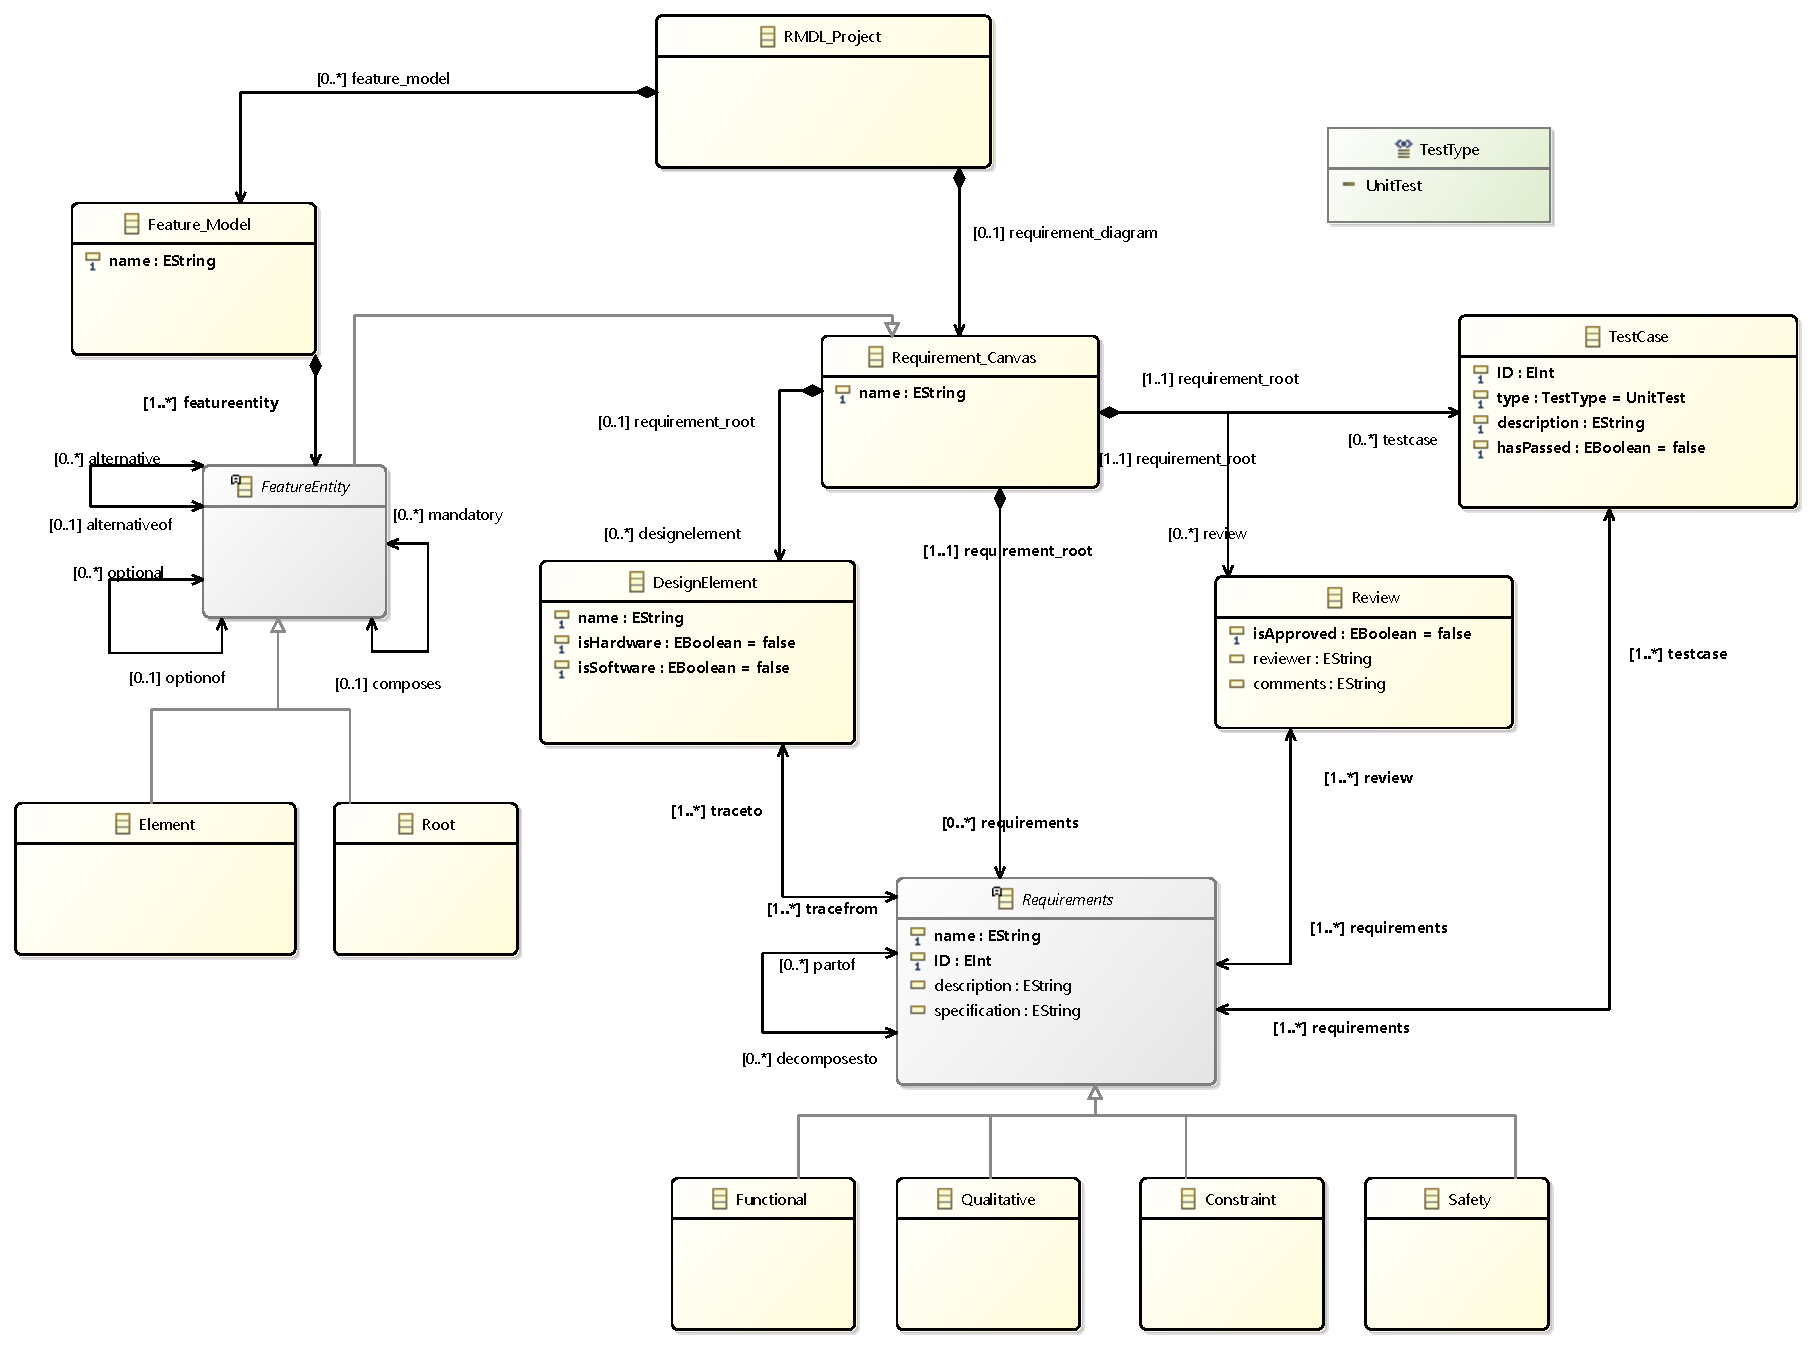
\includegraphics[width=\textwidth]{rmdl.pdf}
	\caption{CyclicL metamodel. Shows the specification for both the requirment canvas and feature modelling portions of CyclicL.}
	\label{fig:metamodel}
\end{figure}

We also added three more classes besides the requirements; \texttt{DesignElement}, \texttt{Review}, and \texttt{TestCase}. The test case and review classes are for verification and validation book-keeping respectively. This is also one of the reasons why we include design elements within the requirement canvas. The test cases are meant to determine if a requirement has been verified against its traced design elements while the review represents if the requirement has been validated. Currently, the verification and validation are expected to happen outside of \tool\ as it was out of scope for initial development. Design elements are also meant to be black boxes as we do not want to pollute our requirement environment with design aspects. We have limited it to determining if a design element is hardware, software, or neither (undetermined when building the requirements or an integrated system). Another reason for having design elements within the requirement canvas is to allow an opportunity for future development for design generation based on the requirements specified in \tool. We also have an enum \texttt{TestType}. This enum allows users to categorize the test users may want to apply to their requirements. At this time in development, only \texttt{UnitTest} is implemented as a type, but more can be added in future revisions.

For the feature modelling portion of the metamodel, the specification is based on the work of Peter H\"{o}fner et al.~\cite{hofner2006feature,hofner2011algebra} which uses set theory as the basis for proving how their feature modelling algebra works. It is also loosely inspired by FeatureIDE~\cite{kastner2009featureide, thum2014featureide} an extremely well-polished feature modelling plugin tool for Eclipse. The main reason we recreated the specification for feature modelling within \tool\ is to explore the implication of using features to encapsulate requirements. This is a key step in the process as this allows for what we dub feature-requirement traceability. As this proposed methodology suggests that features be used to encapsulate requirement to support feature-driven development efforts, having a way of representing that relationship in a formal specification such as a metamodel was impactful both for the development of \tool\ and the development of the concept.

\section{Feature-Requirement Traceability}

The feature-requirement traceability is the main purpose for this methodology. As previous steps have been taken to identify both the features and requirements of the system, this relationship between features and requirements is integral for the process. This relationship is captured by the inheritance connection between the \texttt{Requirement\_Canvas} and the \texttt{FeatureEntity} classes in the metamodel. By allowing every model element in the feature model to double as a requirement canvas, it allows each feature to contain all the model elements requirement for the requirement canvas thus encapsulating the various types of requirements, their associated approvals, and associated design elements.

This relationship allows for several key benefits. First, it allows for direct traceability between the requirements and their respective features. Since every requirement will be `owned' by a feature, we can easily trace the relationship between requirements within a feature, between various features, and within the entire system. Secondly, this modelling approach is more reflective of the relationship that features and requirement have in \ac{FDD} environments allowing more compliance between tolls that support \ac{FDD}. Thirdly, this allows us to model product variance at the requirement level. Allowing for specification of product variance is helpful for reducing unexpected changes and capturing knowledge of anticipated variance in product early in the product lifecycle development. Further, this will support change impact analysis across product variants to support product maintenance. 

Some anticipated downsides to this extension is that it might not be compatible with existing feature model composition approaches. Since every feature element now doubles as a requirement canvas this can break conventional feature composition strategies forcing us to create new ones. Another downside is handling requirements that can be related to multiple features. Due to the encapsulation strategy we are proposing, cross-cutting requirements across features is not supported at this time. There might be ways that users circumvent this which can lead to duplicated or inconsistent requirement across several features. 

\section{Requirement Refinement}

\section{Feature Composition}

\section{Requirement Composition}